\documentclass[11pt]{report}

%-------------------------------------------------------------------------------------------------%

% PAQUETES

\usepackage[a4paper, right = 0.8in, left = 0.8in, top = 0.8in, bottom = 0.8in]{geometry}
\usepackage[utf8]{inputenc}
\usepackage[spanish]{babel}
\usepackage{amsmath,amsfonts,amssymb,amsthm}
\usepackage{multicol}
\usepackage{fouriernc}
\usepackage{enumitem}
\usepackage{mathtools} % Solo uso \underbracket
\usepackage{cellspace, tabularx, booktabs} % Líneas del título
\usepackage{parskip}
\usepackage{pdfpages}
\usepackage{cancel}

%-------------------------------------------------------------------------------------------------%

% AJUSTES GENERALES

\setlist[enumerate]{label={\textit{\alph*})}}

\makeatletter % Para quitar el espacio adicional que el paquete parskip añade al principio y al final de una demostración
\renewenvironment{proof}[1][\proofname]{\par
  \pushQED{\qed}%
  \normalfont \topsep\z@skip % <---- changed here
  \trivlist
  \item[\hskip\labelsep
        \itshape
    #1\@addpunct{.}]\ignorespaces
}{%
  \popQED\endtrivlist\@endpefalse
}
\makeatother

%-------------------------------------------------------------------------------------------------%

% COMANDOS PERSONALIZADOS

\newcommand{\N}{\mathbb N}
\newcommand{\Z}{\mathbb Z}
\newcommand{\Q}{\mathbb Q}
\newcommand{\R}{\mathbb R}
\newcommand{\C}{\mathbb C}

\newcommand{\pars}[1]{\left( #1 \right)} % Paréntesis de tamaño automático
\newcommand{\comment}[1]{}

%-------------------------------------------------------------------------------------------------%

% EJERCICIOS Y SOLUCIONES

\newtheorem{ejercicio}{Ejercicio}
\addto\captionsspanish{\renewcommand*{\proofname}{Solución}}

%-------------------------------------------------------------------------------------------------%

\begin{document}

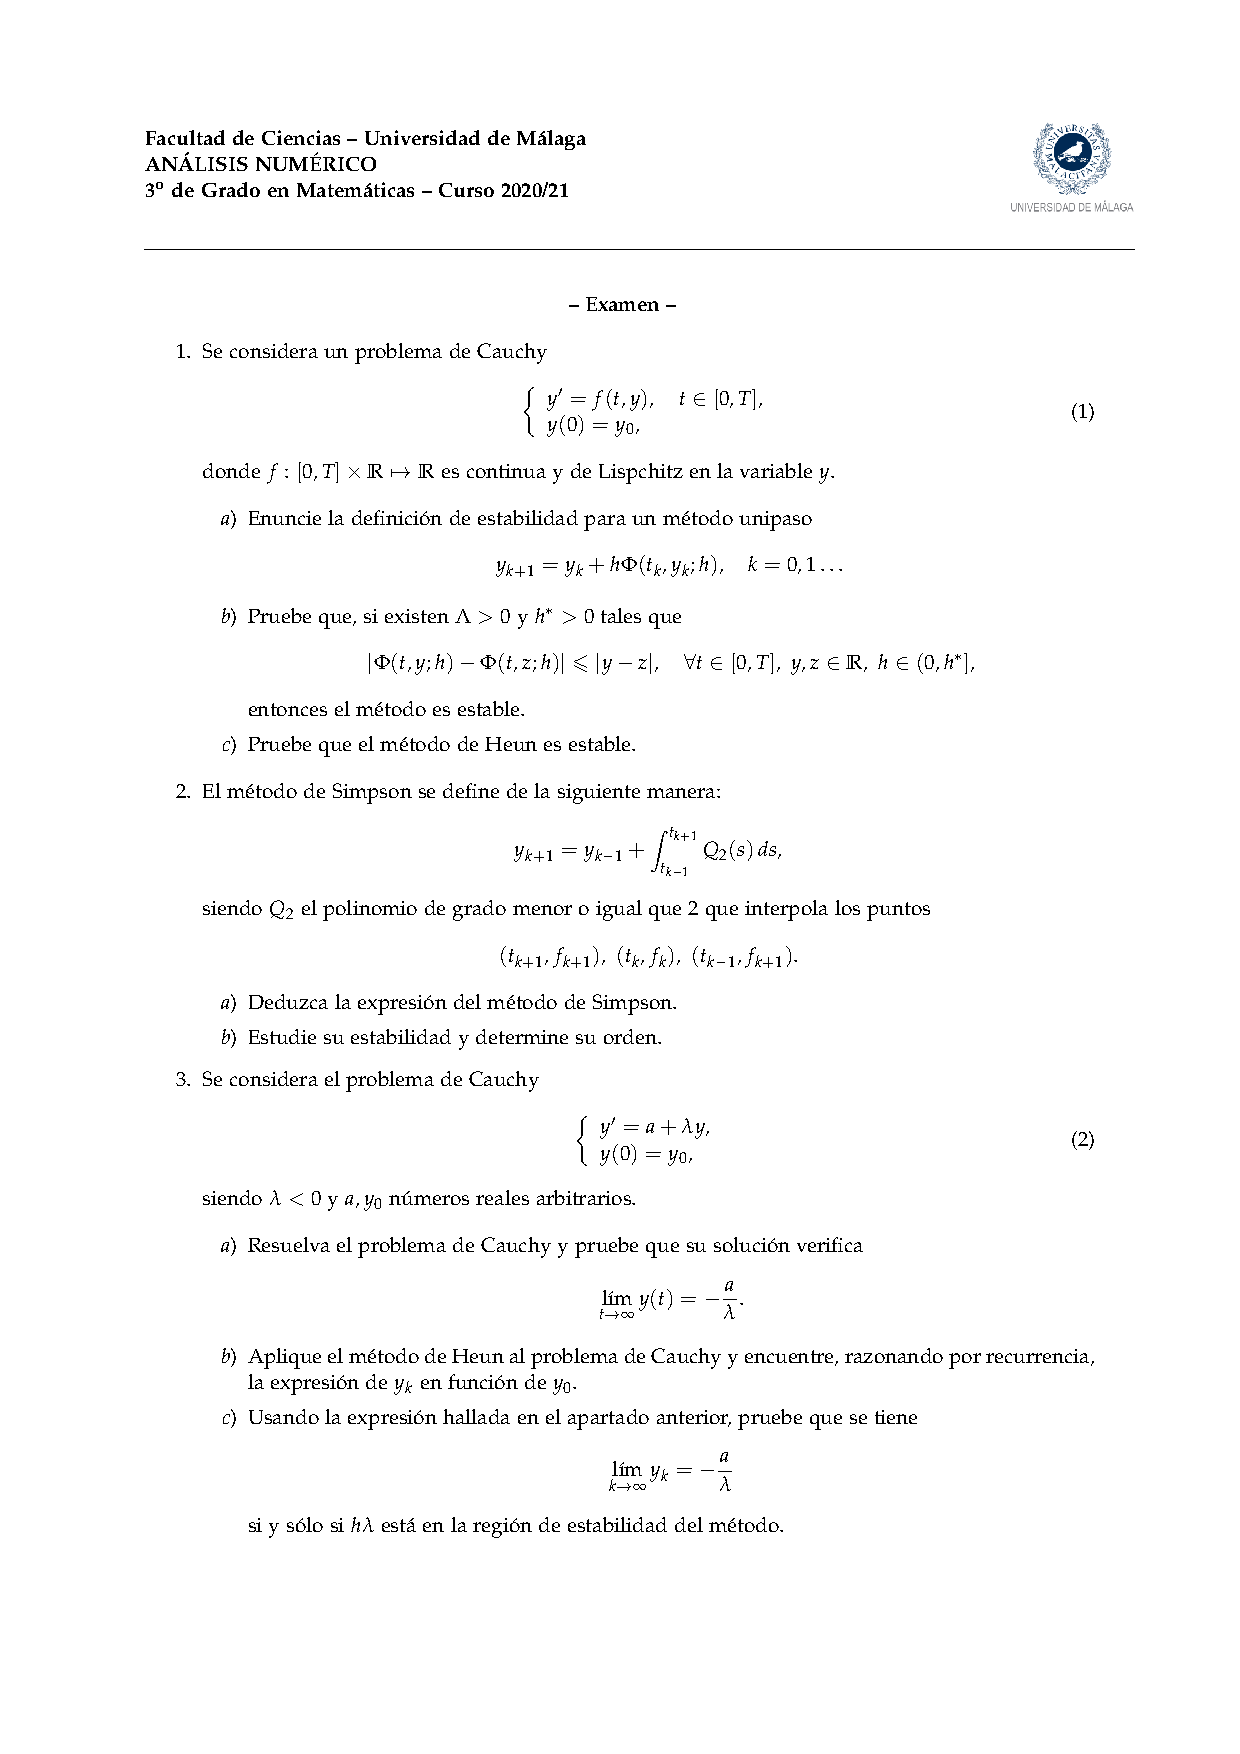
\includepdf[pages=-]{an_examen_2021-09.pdf}

%-------------------------------------------------------------------------------------------------%

% TÍTULO

\begin{center}

	\textbf{$-$ Resolución $-$}

\end{center}

%-------------------------------------------------------------------------------------------------%

\textbf{1.}

\begin{enumerate} 
    \item Se dice que un método unipaso es \emph{estable} si existe una constante $M$ positiva e independiente de $h$ verificando lo siguiente: dados $\{y_k\}_{k=0}^n$, $\{z_k\}_{k=0}^n$, $\{\delta_k\}_{k=0}^{n-1}$ tales que
    \[y_{k+1} = y_k+h\Phi(t_k,y_k,h), \qquad \qquad z_{k+1}=z_k+h\Phi(t_k,z_k,h)+\delta_k\]
    para todo $k = 0,1,\mathellipsis,n-1$, se tiene que
    \[\max_{k=0,1,\mathellipsis,n} |y_k-z_k| \leq M\left(|y_0-z_0|+\sum_{k=0}^{n-1} |\delta_k|\right)\]
    \item Supongamos que existen $\Lambda >0$ y $h^*>0$ con
    \[|\Phi(t,y,h)-\Phi(t,z,h)| \leq \Lambda |y-z|, \qquad \qquad t \in [0,T], \, y,z \in \R, \, h \in (0,h^*]\]
    Veamos que el método es estable. Sean $\{y_k\}_{k=0}^n$, $\{z_k\}_{k=0}^n$, $\{\delta_k\}_{k=0}^{n-1}$ tales que
    \[y_{k+1} = y_k+h\Phi(t_k,y_k,h), \qquad \qquad z_{k+1}=z_k+\Phi(t_k,z_k,h)+\delta_k\]
    para todo $k \in\{ 0,1,\mathellipsis,n-1\}$. Si $k \in \{1,2,\mathellipsis,n\}$,
    \[\begin{aligned}[t]
        |y_k-z_k| &= |y_{k-1}+h\Phi(t_k,y_{k-1},h) -z_{k-1}-h\Phi(t_k,z_{k-1},h)-\delta_k| \\
        &\leq |y_{k-1}-z_{k-1}|+h|\Phi(t_k,y_{k-1},h)-\Phi(t_k,z_{k-1},h)| + |\delta_k| \\
        &\leq |y_{k-1}-z_{k-1}|+h\Lambda |y_{k-1}-z_{k-1}| + |\delta_k| = (1+h\Lambda) |y_{k-1}-z_{k-1}|+|\delta_k| \\
        &\leq  (1+h\Lambda)^2|y_{k-2}-z_{k-2}|+(1+h\Lambda)|\delta_{k-1}|+|\delta_k| \\
        &\leq  (1+h\Lambda)^3|y_{k-3}-z_{k-3}|+(1+h\Lambda)^2|\delta_{k-2}|+(1+h\Lambda)|\delta_{k-1}|+|\delta_k| \\
        &\leq \mathellipsis \\
        &\leq (1+h\Lambda)^k |y_0-z_0|+\sum_{i=0}^k (1+h\Lambda)^i |\delta_{k-i}| \\
        &\leq (1+h\Lambda)^k |y_0-z_0|+(1+h\Lambda)^k\sum_{i=0}^k  |\delta_{k-i}| = (1+h\Lambda)^k\left(|y_0-z_0| +\sum_{i=0}^k |\delta_i|\right) \\
        &\leq  (1+h\Lambda)^k\left(|y_0-z_0| +\sum_{i=0}^{n-1} |\delta_i|\right)
    \end{aligned} \]
    Usando que $e^x \geq 1+x$ para todo $x \in \R$, que $k \leq n$ y que $nh = T$, entonces
    \[|y_k-z_k| \leq e^{kh\Lambda}\left(|y_0-z_0| +\sum_{i=0}^{n-1} |\delta_i|\right) \leq e^{T\Lambda}\left(|y_0-z_0| +\sum_{i=0}^{n-1} |\delta_i|\right)\]
    Para $k = 0$ esta desigualdad sigue siendo cierta. Por tanto,
    \[\max_{k=0,1,\mathellipsis,n} |y_k-z_k| \leq e^{T\Lambda}\left(|y_0-z_0|+\sum_{k=0}^{n-1} |\delta_k|\right),\]
    donde $e^{T\Lambda}$ es una constante positiva e independiente de $h$, concluyéndose que el método es estable.
    \item El método de Heun es el método RK con tablero de Butcher
    
\begin{center}
    \setlength\extrarowheight{2.5pt}
    \begin{tabular}{c|cc}
        0 & 0 & 0 \\
        1 & 1  & 0 \\ \hline
        & 1/2 & 1/2
    \end{tabular}
\end{center}

En otros términos,
\[\left\{\begin{alignedat}{1}
    y_k^{*} &= y_k+hf(t_k,y_k) \\
    y_{k+1} &= y_k+\frac{h}{2}\bigl(f(t_k,y_k)+f(t_k+h,y_k^*)\bigr)
\end{alignedat}\right.\]
Por tanto, la función incremento del método de Heun es 
\[\Phi(t,y,h) = \frac{1}{2}\bigl(f(t,y)+f(t+h,y+hf(t,y))\bigr), \qquad t \in [0,T], \, y \in \R, \, h \in (0,h^*]\]
Sean $y,z \in \R$. Entonces, usando que $f$ es de Lipschitz en la variable $y$ con constante de Lipschitz $L>0$,
\[
\begin{aligned}[t]
|\Phi(t,y,h)-\Phi(t,z,h)| &\leq \frac{1}{2}|f(t,y)-f(t,z)|+\frac{1}{2}|f(t+h,y+hf(t,y))-f(t+h,z+hf(t,z))| \\
&\leq \frac{L}{2}|y-z|+\frac{L}{2}|y+hf(t,y)-z-hf(t,z)| \\
&\leq\frac{L}{2}|y-z|+\frac{L}{2}|y-z|+\frac{hL}{2}|f(t,y)-f(t,z)| \\
&\leq\frac{L}{2}|y-z|+\frac{L}{2}|y-z|+\frac{hL}{2}|y-z| = \left(L+\frac{hL}{2}\right)|y-z|
\end{aligned}
\]
Por el apartado anterior, el método es estable.

\end{enumerate}

\textbf{2.} Véase la segunda relación de ejercicios.

\textbf{3.} 

\begin{enumerate}
    \item La solución general de la ecuación homogénea $y'=\lambda y$ es $y_h(t)=ce^{\lambda t}$, $c \in \R$. Para hallar una solución particular de la ecuación $y'=a+\lambda y$, recurrimos al método de variación de los parámetros: se busca una solución de la forma $y_p(t)=c(t)e^{\lambda t}$. Se tiene que
    \[\begin{aligned}[t]
        y_p(t)=c(t)e^{\lambda t} \textup{ es solución de } y'=a+\lambda y &\iff c'(t)e^{\lambda t} +\lambda c(t)e^{\lambda t} = a+\lambda c(t)e^{\lambda t} \\
        &\iff c'(t)=ae^{-\lambda t}
    \end{aligned} 
    \]
    Podemos tomar, por ejemplo, $c(t)=-\frac{a}{\lambda}e^{-\lambda t}$, luego $y_p(t)=-\frac{a}{\lambda}$ y por tanto la solución general de $y'=a+\lambda y$ es $y(t)=ce^{\lambda t}-\frac{a}{\lambda}$, $c \in \R$. Imponiendo $y(0)=y_0$ se obtiene $c = y_0+\frac{a}{\lambda}$, luego
    \[y(t)=\left(y_0+\frac{a}{\lambda}\right)e^{\lambda t}-\frac{a}{\lambda}\]
    es la única solución del problema dado, que por ser $\lambda <0$ verifica
    \[\lim_{t \to \infty} y(t)=-\frac{a}{\lambda}\]
    \item El método de Heun para este problema es
    \[\left\{\begin{alignedat}{1}
    y_k^{*} &= y_k+h(a+\lambda y_k), \\
    y_{k+1} &= y_k+\frac{h}{2}\bigl(a+\lambda y_k+a+\lambda y_k^*\bigr),
\end{alignedat}\right.\]
es decir,
\[
\begin{aligned}[t]
    y_{k+1} &= y_k+\frac{h}{2}\bigl(2a+\lambda y_k+\lambda y_k+\lambda h a + \lambda^2h y_k\bigr) = y_k+ah+\lambda y_kh+\frac{a\lambda}{2}h^2+\frac{\lambda^2y_k}{2}h^2 \\
    &= \left(1+\lambda h +\frac{\lambda^2h^2}{2}\right)y_k + ah+\frac{a\lambda}{2}h^2
\end{aligned}
\]
Razonando por recurrencia,
\[
\begin{aligned}[t]
    y_k &= \left(1+\lambda h +\frac{\lambda^2h^2}{2}\right)y_{k-1} + ah+\frac{a\lambda}{2}h^2 \\
    &= \left(1+\lambda h +\frac{\lambda^2h^2}{2}\right)^2y_{k-2} + \left(1+\lambda h +\frac{\lambda^2h^2}{2}\right)\left(ah+\frac{a\lambda}{2}h^2\right)+\left(ah+\frac{a\lambda}{2}h^2\right) \\
    &= \mathellipsis \\
    &=  \left(1+\lambda h +\frac{\lambda^2h^2}{2}\right)^ky_{0}+ \left(ah+\frac{a\lambda}{2}h^2\right)\sum_{i=0}^k\left(1+\lambda h +\frac{\lambda^2h^2}{2}\right)^i
\end{aligned}
\]
\item Se observa que $y_k$ tiene límite cuando $k \to \infty$ si y solo si
\[\left|1+\lambda h+\frac{\lambda^2h^2}{2}\right| < 1\]
Se comprueba fácilmente que la función de estabilidad absoluta del método de Heun es 
\[R(\hat{h}) = 1+\hat{h}+\frac{\hat{h}^2}{2}\]
Se concluye que $y_k$ tiene límite cuando $k \to \infty$ si y solo si $\lambda h \in \{\hat{h} \in \C \colon |R(\hat{h})| < 1\} = D_A$ y, en ese caso,
\[
\begin{aligned}[t]
\lim_{k \to \infty} y_k &=  \left(ah+\frac{a\lambda}{2}h^2\right)\sum_{i=0}^\infty\left(1+\lambda h +\frac{\lambda^2h^2}{2}\right)^i = \left(ah+\frac{a\lambda}{2}h^2\right) \frac{1}{1-1-\lambda h -\frac{\lambda^2h^2}{2}} \\
&= -\left(ah+\frac{a\lambda}{2}h^2\right) \frac{1}{\lambda h +\frac{\lambda^2h^2}{2}} = -\frac{a}{\lambda}\left(h+\frac{\lambda}{2}h^2\right) \frac{1}{ h +\frac{\lambda h^2}{2}} = -\frac{a}{\lambda}
\end{aligned}
\]
\end{enumerate}

\textbf{4. } Ejercicios muy similares a este se han hecho ya unas cuantas veces.
\end{document}